%!TEX TS-program = xelatex
%!TEX encoding = UTF-8 Unicode

\documentclass[a4paper,10pt]{article}

\usepackage[a4paper,textwidth=42em,tmargin=37mm,bmargin=10mm]{geometry}
\usepackage[dvipsnames]{xcolor}
\usepackage{calc}
\usepackage{amsmath,xltxtra,xunicode}
\usepackage{titlesec}
\usepackage{fontspec}
\usepackage{wasysym,oz,pxfonts,txfonts}
\usepackage{datetime2}



\usepackage[PunctStyle=plain,RubberPunctSkip=false,CJKglue=\hskip 0pt,CJKecglue=\hskip 4pt plus 20pt]{xeCJK}
\usepackage{xeCJKfntef}
\XeTeXlinebreaklocale "zh"
\XeTeXlinebreakskip = 0pt plus 1pt

% =========================================
\usepackage{everypage}
\usepackage{listings}
\usepackage{paralist}
\usepackage{enumerate}
\usepackage{enumitem}
\usepackage{tocloft}
\usepackage{longtable}
\usepackage{tabu}
\usepackage{makecell}
\usepackage{qrcode}
\usepackage{graphicx}
\usepackage{tikz}
\usepackage{eso-pic}
\graphicspath{ {/home/neruthes/DEV/ntexlibs/pic} }
\usepackage{fontawesome5}
\usepackage{multirow}
\usepackage{multicol}
\usepackage{ragged2e}
\usepackage{tcolorbox}
\setmainfont{Nimbus Roman}
\setromanfont{Nimbus Roman}
\setsansfont{Inter}
\setmonofont{ocrb10}
\setCJKmainfont{Noto Sans CJK SC}
\setCJKromanfont{Noto Serif CJK SC}
\setCJKsansfont{Noto Sans CJK SC}
\setCJKmonofont{Noto Sans CJK SC}

\setdefaultleftmargin{2em}{2em}{1em}{1em}{1em}{1em}

\newcommand{\kaifamily}[0]{\CJKfontspec{FandolKai}}

\title{}
\author{}
\date{}
\pagestyle{plain}
% =========================================

% =========================================
% START CORPORATION CONFIG
\setlength{\parindent}{0pt}
\setlength{\parskip}{1pt}
\setlength{\baselineskip}{12pt}
% END CORPORATION CONFIG
% =========================================

% =========================================
% START COMMON STYLESHEET
% Table
\renewcommand\theadalign{l}
\renewcommand\theadfont{\sffamily\bfseries}
% Font Size

% END COMMON STYLESHEET
% =========================================


\linespread{1.1}




\newcommand{\tval}[1]{{\hspace{14pt}\ttfamily\upshape\mdseries\small\textcolor{red}{#1}}}
\newcommand{\bondkeyval}[2]{
	{\small#1} & {\tval{#2}}
}



% ==============================================
% Magic. Do not touch.
% ==============================================
\makeatletter


\def\makeBondPage{
\@ifnextchar{[}
{\@makeBondPage}
{\@makeBondPage[]}
}

\def\@makeBondPage[#1]#2{
	\setkeys{makeBondPage}{#1}

	\color{blue!12!black!80!white}
	\begin{minipage}{\textwidth}
		\center

		\baselineskip=27pt
		% {\color{blue!12!black!80!white}\Huge\ttfamily\bfseries\fontspec[LetterSpace=6]{Elsie Black}TREASURY\linebreak BOND}
		{\color{blue!12!black!80!white}\Huge\ttfamily\bfseries\fontspec[LetterSpace=12]{Major Mono Display}treasury\linebreak bond}\par
		\vspace{15pt}

		{{\ttfamily\large\color{red}S/N \bond@sn}}
		% \vspace{10pt}

		% {#1}
	\end{minipage}
	\vspace{40pt}

	\rmfamily

	\tabulinesep=11pt
	% \tabcolsep=0pt

	\begin{minipage}{\linewidth}
		\center

		\large

		{{
\includegraphics[width=42mm]{neruthes-grandseal-core.png}}}
		\vspace{25pt}

		{\Huge\fontspec{Realtime Rounded}\bfseries NERUTHES}
		\vspace{20pt}

		\sffamily\normalsize
		\baselineskip=16pt
		\MakeUppercase{for value received}\par
		\MakeUppercase{promises to pay to the bearer}\par
		\MakeUppercase{the sum of}

		\vspace{20pt}

		{\Huge\bfseries\fontspec{Justice}\bond@value}

		{\underline{\hspace{0.4\linewidth}}}
		\vspace{35pt}

		\sffamily\small
		\tabcolsep=0pt
		\tabulinesep=12pt
		% \fontspec{Erato}
		\begin{tabu} {lXlX}
			\hline
			\bondkeyval{DATE OF ISSUE}{\bond@dateDeal} &
			\bondkeyval{MATURITY DATE}{\bond@dateMature} \\
			\hline
			\bondkeyval{YIELD RATE}{\bond@yieldRate}   &
			\bondkeyval{CURRENCY}{\bond@currency}                 \\
			\hline
		\end{tabu}
	\end{minipage}
	\vspace{25pt}

	\sffamily
	\tabcolsep=5pt
	\begin{tabu} {X[c]X[c]}
		{}                             & {}                         \\
		{}                             & {}                         \\
		{}                             & {}                         \\
		% {\hrule} & {\hrule} \\
		% \hline
		{\hrule\vspace{5pt} SIGNATURE} & {\hrule\vspace{5pt} STAMP} \\
	\end{tabu}




}

\define@key{makeBondPage}{sn}[????]{\def\bond@sn{#1}}
\define@key{makeBondPage}{value}[????]{\def\bond@value{#1}}
\define@key{makeBondPage}{dateDeal}[????]{\def\bond@dateDeal{#1}}
\define@key{makeBondPage}{dateMature}[????]{\def\bond@dateMature{#1}}
\define@key{makeBondPage}{yieldRate}[????]{\def\bond@yieldRate{#1}}
\define@key{makeBondPage}{currency}[????]{\def\bond@currency{#1}}

\makeatother







\pagestyle{empty}


\AddToShipoutPictureBG*{%
	\put(1mm,2.7mm){%
		{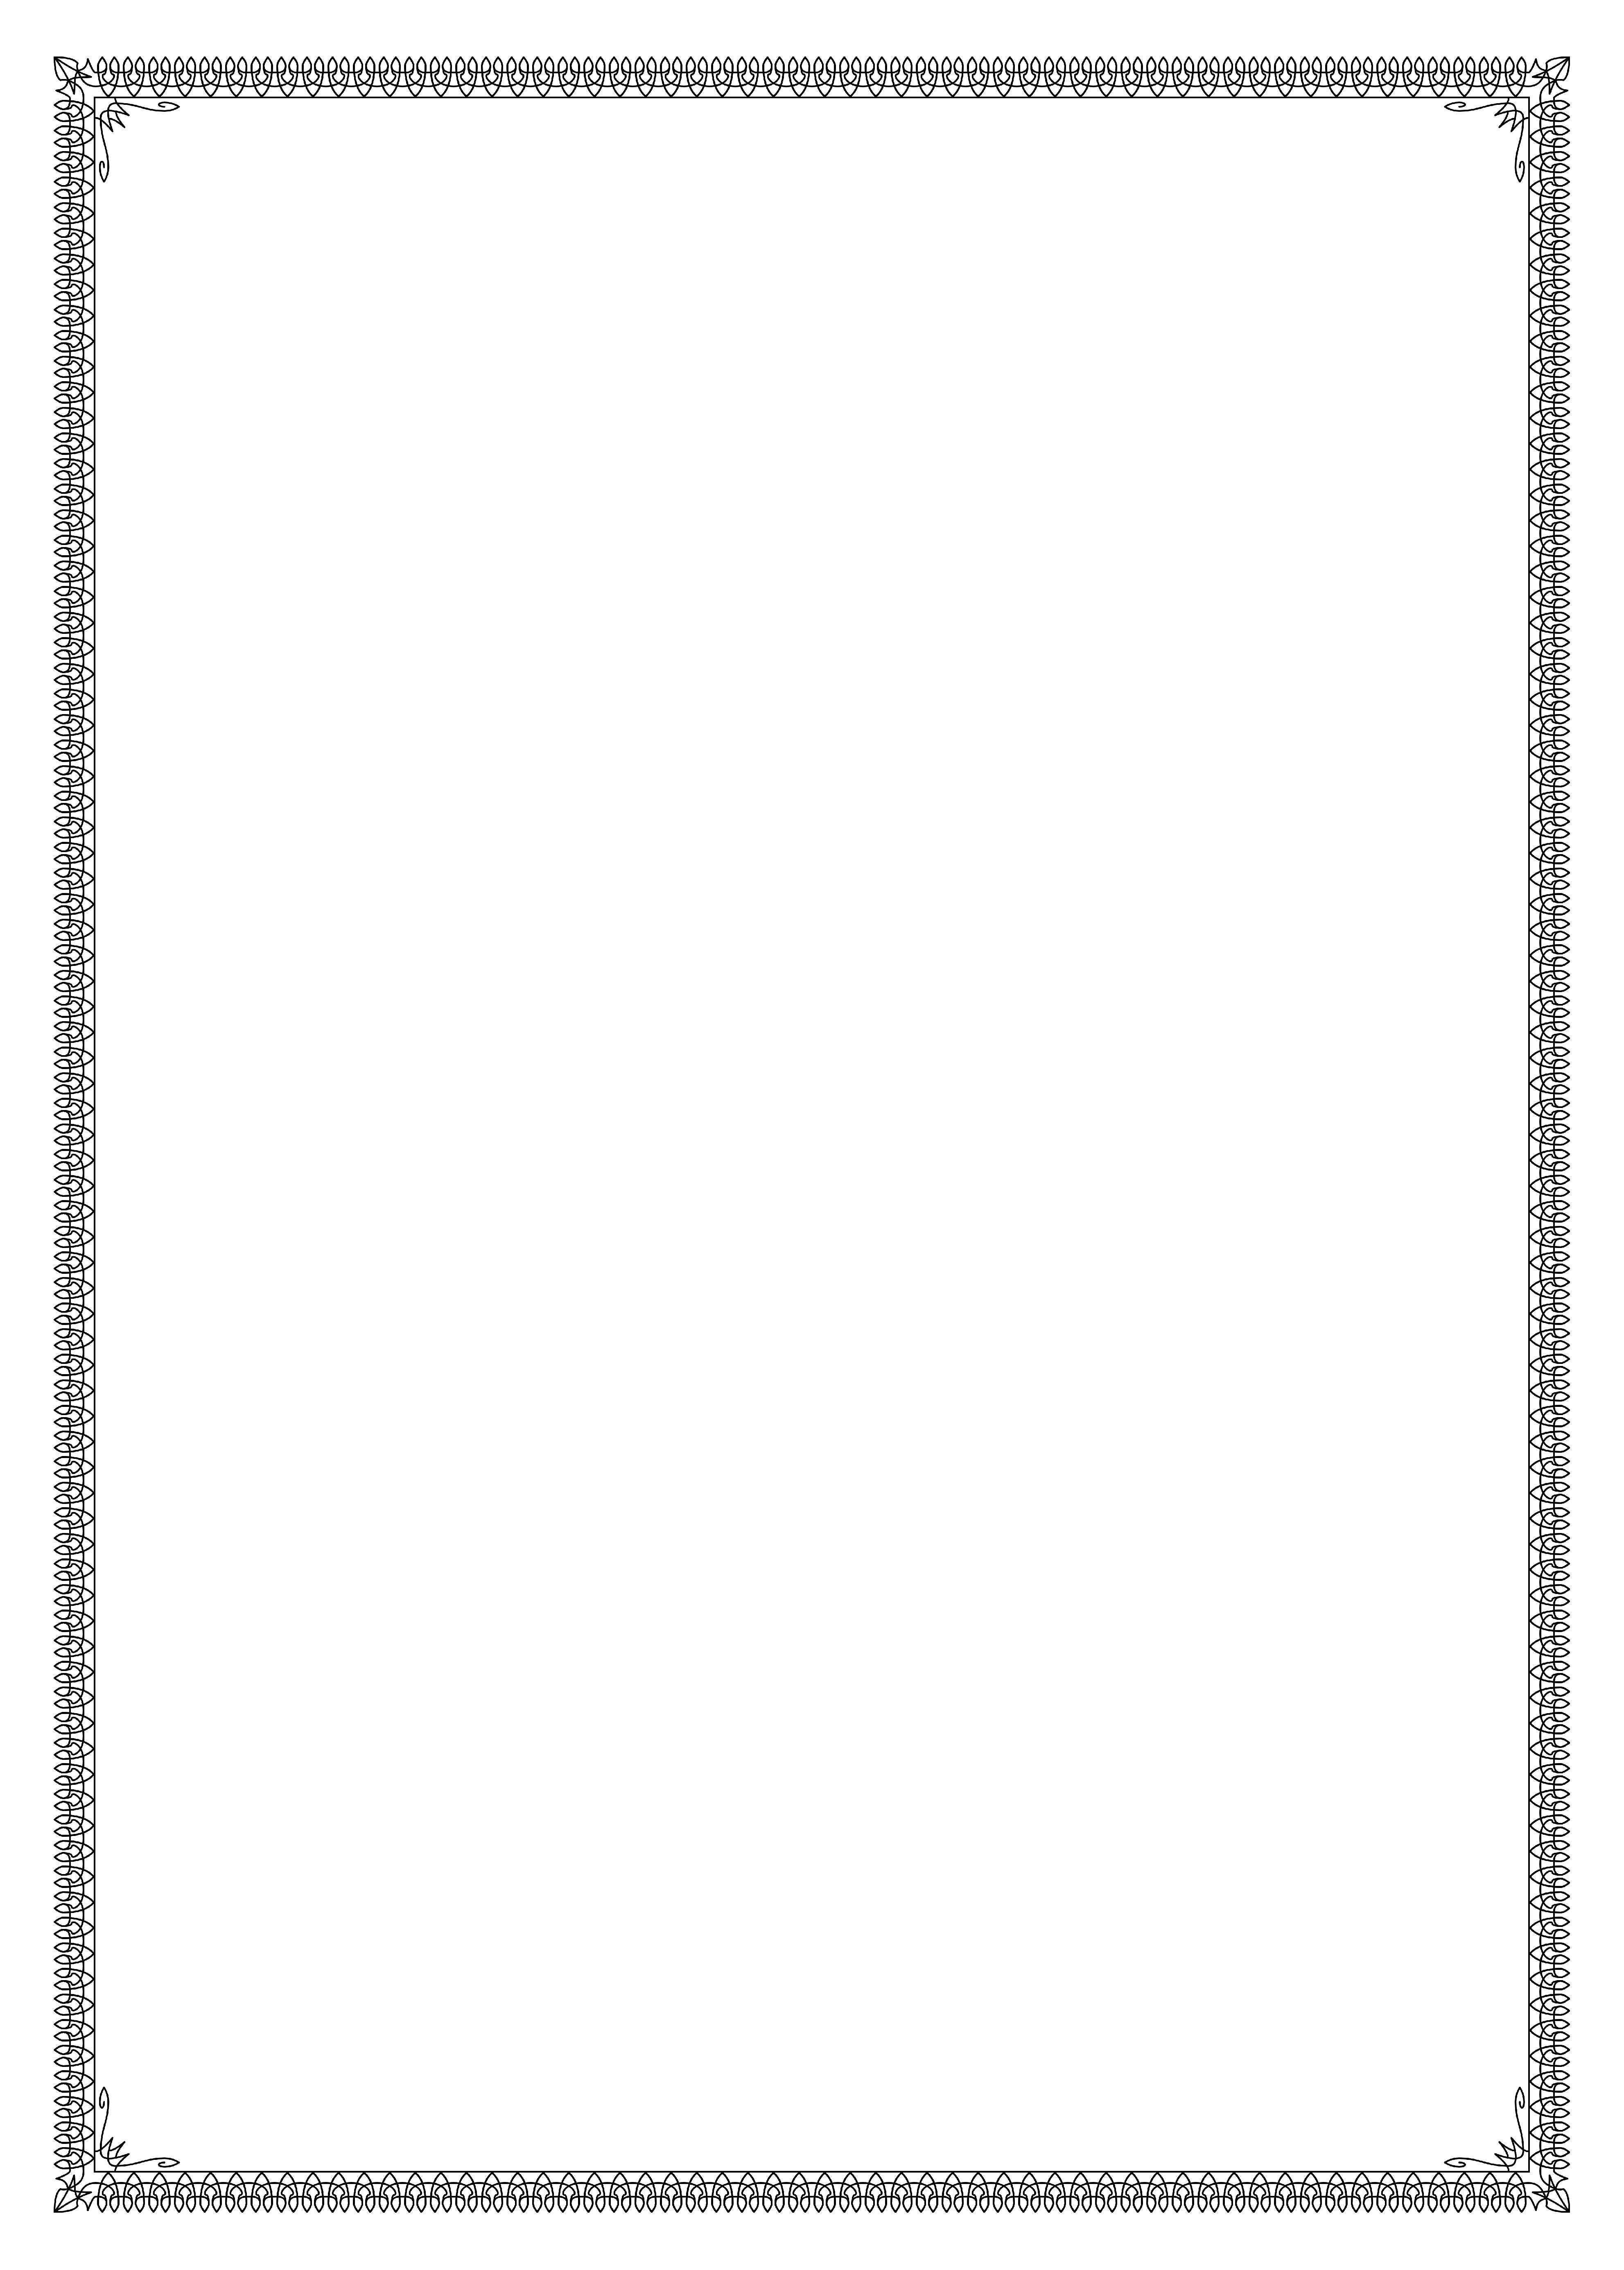
\includegraphics[width=\paperwidth-2mm]{neoparia/N-PageBorder.eps}}%
	}%
}
\AddToShipoutPictureBG*{%
	\put(-43.5mm,0mm){%
		{\includegraphics[width=\paperheight,height=\paperheight]{neoparia/pattern/EP-4-black_20p.png}}%
	}%
}
